\documentclass{article}

% if you need to pass options to natbib, use, e.g.:
%     \PassOptionsToPackage{numbers, compress}{natbib}
% before loading neurips_2021

% ready for submission
\usepackage[preprint]{neurips_2021}

% to compile a preprint version, e.g., for submission to arXiv, add add the
% [preprint] option:
%     \usepackage[preprint]{neurips_2021}

% to compile a camera-ready version, add the [final] option, e.g.:
%     \usepackage[final]{neurips_2021}

% to avoid loading the natbib package, add option nonatbib:
%    \usepackage[nonatbib]{neurips_2021}

\usepackage[utf8]{inputenc} % allow utf-8 input
\usepackage[T1]{fontenc}    % use 8-bit T1 fonts
\usepackage[colorlinks=true]{hyperref}       % hyperlinks
\usepackage{url}            % simple URL typesetting
\usepackage{booktabs}       % professional-quality tables
\usepackage{amsfonts}       % blackboard math symbols
\usepackage{nicefrac}       % compact symbols for 1/2, etc.
\usepackage{microtype}      % microtypography
\usepackage{xcolor}         % colors
\usepackage{graphicx}
\usepackage{subcaption}

\title{Predicting Student Performance\\ from Admissions and Historical Performance Data}

% The \author macro works with any number of authors. There are two commands
% used to separate the names and addresses of multiple authors: \And and \AND.
%
% Using \And between authors leaves it to LaTeX to determine where to break the
% lines. Using \AND forces a line break at that point. So, if LaTeX puts 3 of 4
% authors names on the first line, and the last on the second line, try using
% \AND instead of \And before the third author name.

\author{%
  Alexander Panfilov\\
  Matrikelnummer 5990087\\
  \texttt{alexander.panfilov@student.uni-tuebingen.de} \\
  \And
  Evgenii Kortukov\\
  Matrikelnummer 5994382\\
  \texttt{evgenii.kortukov@student.uni-tuebingen.de} \\
}

\begin{document}

\maketitle

\begin{abstract}
   We use a private dataset of anonymized data from students of
one Russian University to assess how well student performance can be
predicted from this data. The dataset contains admission data (state exam results, subject competition prizes, and sociodemographic
information) and data of students’ university performance. We conduct statistical testing, apply linear
regression and dimensionality reduction techniques to provide a proof of concept of a student embedding.
\end{abstract}

\section{Introduction}
\label{sec:intro}
With the advent of MOOCs and personalized learning solutions universities have to adapt to maintain a competitive advantage and attract potential students. A promising innovation would be to implement data-driven personalized study plans tailored to the needs of every student. Such an approach has to rely on a sufficiently informative and predictive model of a student. Our main contribution is to provide a proof of concept. We show that available data is sufficient to construct embeddings with predictive power and provide examples of possible predictions.

\section{Data}
\label{sec:data}
We perform our analysis on a dataset that contains information on approximately 20000 bachelor students of one Russian University. It contains a set of anonymized features which can describe a particular student. Students contributed to the dataset voluntarily and gave written consent for using their data for research purposes. Data consists of 2 main parts.

\textbf{Admission data} is the information that University knows about a student at the time of admission. In order to apply to University candidates must possess a school-leaving certificate and provide at least one of the following things: 

  \underline{State exam results}: Each program offers a limited number of study places without a tuition fee on a competitive basis. Students with scores below the passing threshold can still be admitted, but on a tuition fee basis;
  \underline{School olympiads results}: Prize holders of subject olympiads can be admitted to Universities without state exam results;
  \underline{In-University exam results}: In special cases University can establish its own inner exams. These exams are taken by foreign applicants who cannot provide state exam results.

Thus, admission data contains exam results or olympiads, chosen faculty and program, fact of paying the tuition fee, country of origin and home region.

Universities employ this data to obtain the most talented students. Before the application period professors visit schools which usually have high exam results or prominent amount of olympiad winners and agitate schoolchildren to apply to their University. This recruitment process can be optimized with the help of data by recruiting from regions with high state exam result: in Figure \ref{fig:mapinf} and Figure \ref{fig:mapmath} we can see a heatmap of mean state exams results of the European part of Russia. Surprisingly the highest scores are not observed in the St. Peterburg's or Moscow's metropolitan areas, as one might expect.

\begin{figure}[t!]
  \centering 
  \begin{subfigure}{0.49\textwidth}
    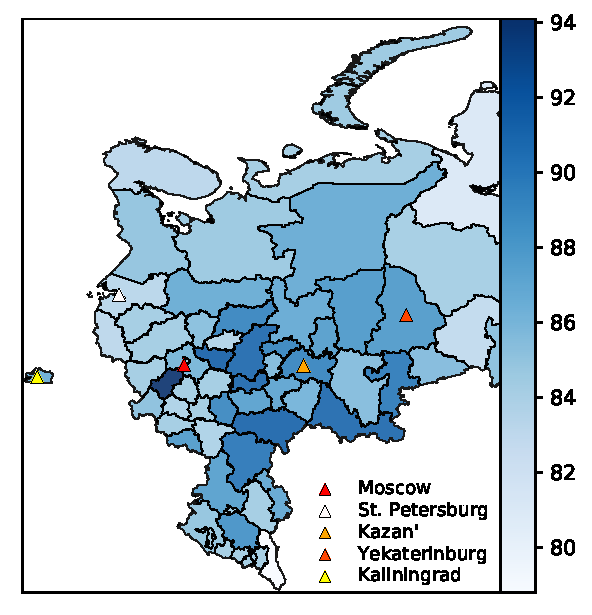
\includegraphics[width=\linewidth]{../gfx/map_informatics.pdf}
    \caption{Mean informatics state exam results}
    \label{fig:mapinf}
  \end{subfigure} 
  \begin{subfigure}{0.49\textwidth}
    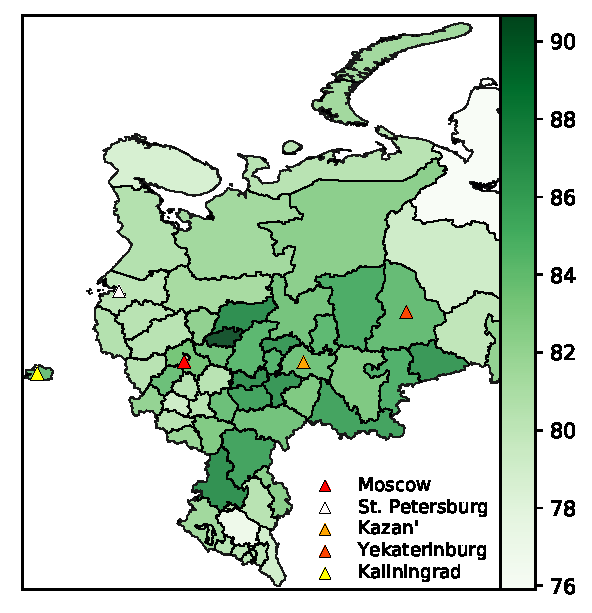
\includegraphics[width=\linewidth]{../gfx/map_math.pdf}
    \caption{Mean mathematics state exam results}
    \label{fig:mapmath}
  \end{subfigure}
  \begin{subfigure}{0.9\textwidth}
    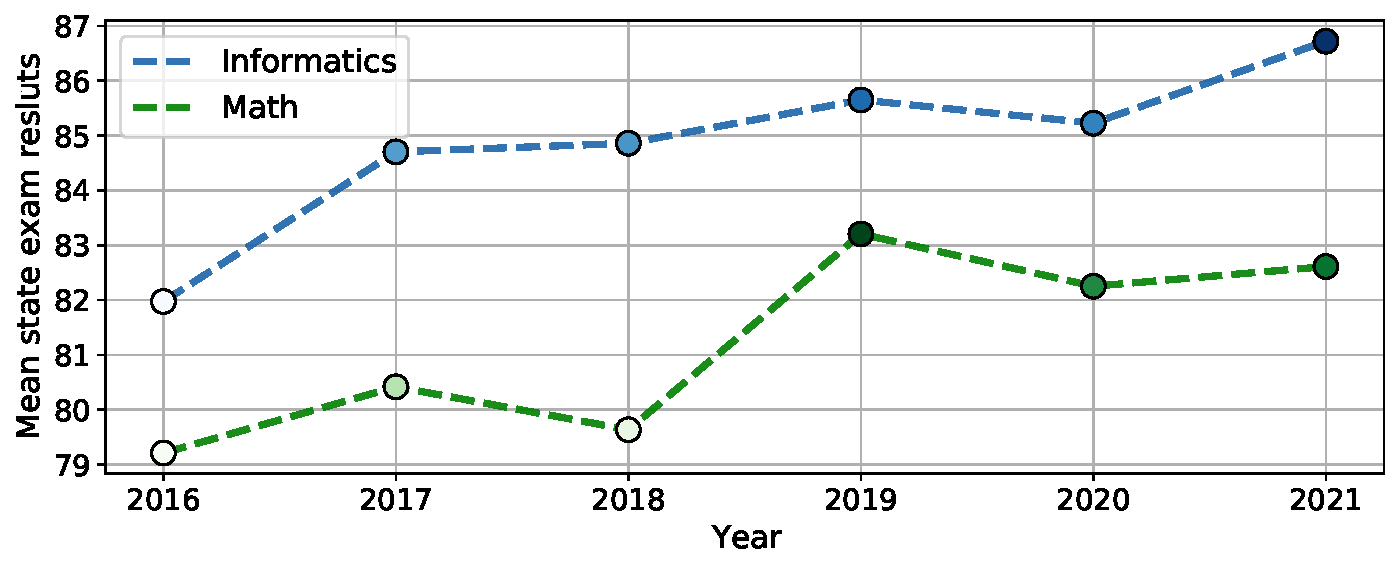
\includegraphics[width=\linewidth]{../gfx/ege_trend.pdf}
    \caption{Mean admitted state exam results over years}
    \label{fig:egetrend}
  \end{subfigure}\hfil
  \captionsetup{belowskip=-10pt}
  \caption{Geographical distribution of the state exam results and trend for the last 5 years.}
\end{figure}

\textbf{Per-semester student performance data} contains following features: GPA, number of failed exams, student group and faculty (which student may change during studies). Also, this data provides some possible target-features: fact of the successful graduation or fact of obtaining \textit{summa cum laude}.

%\section{Preprocessing}
%\label{sec:preprocess}

The dataset posed two main difficulties: large number of missing values and categorical features, which are problematic for linear models. 

%Some of the missing values were filled using complementary columns' information, from which you can obtain the correct value of the feature. Otherwise, categorical features were one-hot encoded with setting a missing value as a separate feature value; one-hot encoding were used to not imply an order for non-ordered features. Missing values for numerical features (mainly early year state exams) were filled with median feature value for the next known year, because median changes less drastically then mean as shown in Section \ref{sec:data}.


\section{Hypothesis testing}
\label{sec:hypothesis}
University admission offices provide benefits to olympiad winners in the admission process. This rests on an assumption that they tend to perform better at the university level.
We seek to justify this approach with data and also motivate further study. The metric of university level performance we use is successful graduation from a study program. We test the null-hypothesis that olympiad winners have the same probability of successfully graduating from university as regularly admitted students.

Our dataset includes 13109 bachelor students who either graduated or dropped out. The admission type is known only for a subset of students. There are \textbf{383} olympiad winners in this subset and \textbf{1275} regularly admitted students. We model each group of students as a series of independent identical Bernoulli experiments with unknown success probability $\pi$. To estimate this quantity we use Bayesian inference.

Let $X_o$ be the set of $n_o = 383$ datapoints of olympiad winners with $m_o = 291$ successful graduates. Then $X_r$ - set of $n_r = 1275$ regularly admitted students with $m_r = 912$ successful graduates.
We want to estimate the probabilities of graduation in both groups $\pi_o$ and $\pi_r$. Using binomial likelihood we get that the posterior distribution over $\pi$ is then Beta distribution $\mathcal{B}(\pi ; m+1,n-m+1)$. This leads us to a \textit{maximum a posteriori} estimate of
$\hat{\pi_o} = 0.760$ and
$\hat{\pi_r} = 0.715$. Figure \ref{fig:test_1} shows the posterior distributions.
Under our model we can say that with 95\% probability $\pi_o$ lies in the interval $[0.714;0.800]$ and $\pi_r$ lies in the interval $[0.690;0.739]$.

Now we test the hypothesis $\mathcal{H}_0$: \textit{"Olympiad winners have the same probability of successful graduation as students admitted under the regular procedure."}. Note, that: 1. Under the null hypothesis $\mathcal{H}_0$ we have $\pi_r = \pi_0 = \pi$. The likelihood of observing $m_o$ successfully graduated olympiad winners given a particular probability $p(m_o| \pi)$ follows a binomial distribution. 2. The previously achieved Beta-posterior over $\pi$ now acts as a prior, so $ p(\pi | m_r, n_r) = \mathcal{B}(\pi;m_r+1, (n_r - m_r) + 1)$. 3. To find the probability of observing $m_o$ successfully graduated olympiad winners under the null hypothesis we marginalise over $\pi$ $p(m_o | \mathcal{H}_0) = \int p(m_o | \pi) p(\pi | m_r, n_r)\,d\pi$

This results in Beta-binomial distribution. \cite{hyp_testing} It is depicted in Figure \ref{fig:test_2}. 
We compute the probability of seeing $m_o$ or more successfully graduated olympiad winners under the null hypothesis and achieve the p-value of $0.037 < 0.05$ which leads us to reject the null hypothesis.

We conclude that olympiad winners and regularly admitted students have statistically significant differences in graduation probability. This warrants further study of other differences in performance between these two groups.

\begin{figure}[t!]
  \centering 
  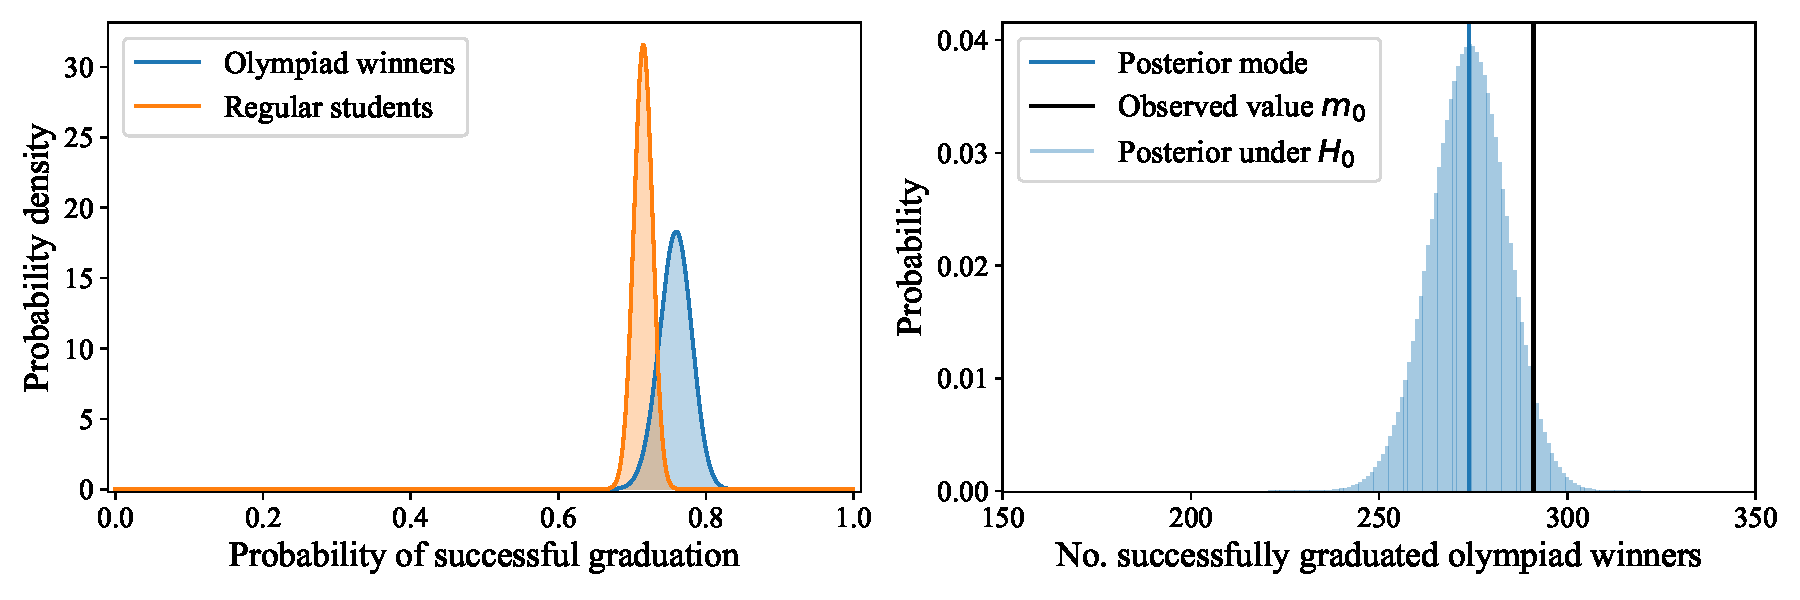
\includegraphics[width=1\linewidth,trim={0.5cm 0 0 0}]{../gfx/testing_fig.pdf}
  \hfill
  \begin{subfigure}{0.48\textwidth}
    \centering
    \caption{Posterior distributions of successful graduation probability $\pi$ for each group of students.}
    \label{fig:test_1}
  \end{subfigure} 
  \hfill
  \begin{subfigure}{0.49\textwidth}
    \centering
    \caption{Posterior distribution of successfully graduated student count under the null hypothesis $H_0$ and the observed count in the olympiad winners group}
  \label{fig:test_2}
  \end{subfigure}
  \hfill
  \captionsetup{belowskip=-15pt}
  \caption{Hypothesis testing results.}
  \label{fig:testing}
  
\end{figure}



\section{Dimensionality reduction}
\label{sec:reduction}
We evaluate how representative is the proposed student embedding. As shown in \ref{sec:hypothesis}, there are significant differences between some groups of students. We assume that if embedding is representative enough, we may visually distinguish graduated and dropped out groups of students in the 2D projection of the embedding. For this purpose we used PCA and t-SNE \cite{van2008visualizing} algorithms. Although the groups are indistinguishable in the subspace of the first two principal components (Figure \ref{fig:pca}), some structure can clearly be observed when using t-SNE algorithm (Figure \ref{fig:tsne}). There is a top red cluster with most of the dropped out students, whereas the right green clusters contain mainly graduated students. Other clusters in picture are more mixed with the prevalence of graduated students.

\begin{figure}[t!]
  \centering 
  \begin{subfigure}{0.49\textwidth}
    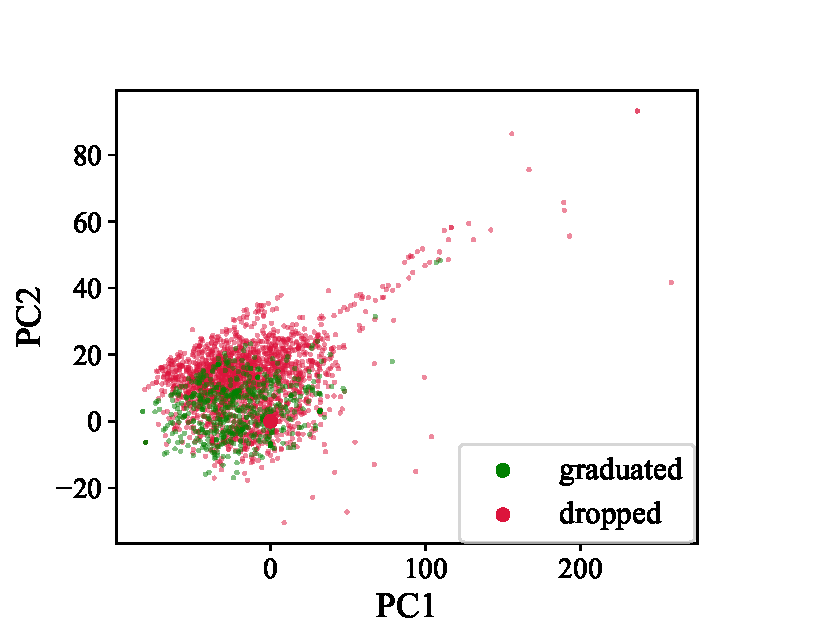
\includegraphics[width=\linewidth]{../gfx/pca.pdf}
    \caption{PCA}
    \label{fig:pca}
  \end{subfigure} 
  \begin{subfigure}{0.49\textwidth}
    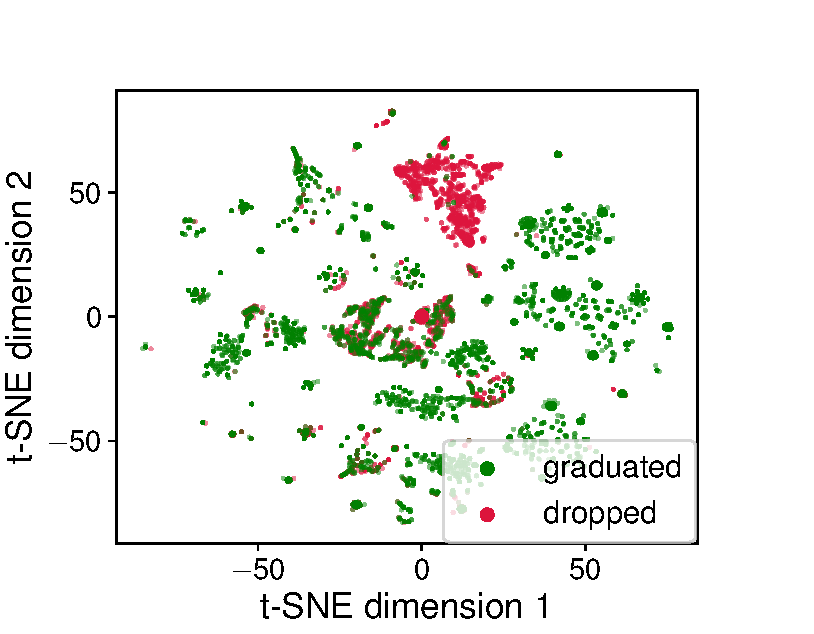
\includegraphics[width=\linewidth]{../gfx/tsne.pdf}
    \caption{t-SNE}
    \label{fig:tsne}
  \end{subfigure}
  \captionsetup{belowskip=-10pt}
  \caption{Dimensionality reduction visualisation.}
  \label{fig:reduction}
\end{figure}

\section{Regression}
We show how student performance can be predicted from admission data. Features described in \ref{sec:data} are independent variables, the response variable is average grade in the first semester. We standardize the data and apply linear regression with L1 regularization \cite{lasso}. The obtained results can be seen in Table \ref{table_regression}. Grades range from 2.0 to 5.0. The achieved accuracy is enough, for example, to identify students who might need additional help or counselling, but not enough for personalized recommendations. Sub-optimal performance might be due to instability of exam results between years \ref{fig:egetrend} and large number of missing values in the data \ref{sec:data}. 

\begin{table}[h!]
\captionsetup{justification=centering}
\centering
\caption{RMSE for predicting grades from admission data. Grades range from 2.0 to 5.0}
\begin{tabular}{ |c||c|c|c| } 
 \hline
 Predicted year & 2015 & 2016 & 2017 \\ 
 \hline
 RMSE & 0.520 & 0.581 & 0.589 \\
 \hline
\end{tabular}
\label{table_regression}
\end{table}

\section{Ethical considerations}
Implementing a system of this kind raises a number of  ethical questions. First,it poses privacy concerns. Participation must be fully voluntary and students should be provided same opportunities regardless of whether they gave out their data. Second, human supervision is needed to make sure that results of using the system are aligned with student values. Lastly, it is vital to make sure that the achieved model does not put groups of people at a disadvantage.
We believe that given a careful data usage strategy, such a system can be very beneficial to both universities and students.

\section{Conclusion}
We have shown that it is possible to create a predictive student model from admission and semester performance data. Such a model can be used to predict future performance of a student.
% bibliography
\bibliographystyle{plain}
\bibliography{bibliography}

\end{document}
